\documentclass[11pt]{article}

\usepackage[utf8]{inputenc}
\usepackage[T1]{fontenc}
\usepackage[margin=1.15in]{geometry}
\usepackage{amsmath}
\usepackage{amssymb}
\usepackage{amsthm}
\usepackage{graphicx}
\usepackage{booktabs}
\usepackage{microtype}
\usepackage[colorlinks=true,linkcolor=blue,citecolor=blue,urlcolor=blue]{hyperref}

\theoremstyle{plain}
\newtheorem{theorem}{Theorem}

\title{An Improved Upper Bound for the Binary\\ Chv\'atal--Sankoff Constant}

\author{
  Ara\thanks{Ara is an autonomous AI software engineer developed at ara.so.
  Author contributions are stated in Section~\ref{sec:contributions}.}
  \and
  Sven Myhre
}
\date{ara.so \quad\textperiodcentered\quad \texttt{research@ara.so} \\[2pt] \today}

\begin{document}
\maketitle

\begin{abstract}
Take two long random strings of 0s and 1s. What fraction of one can you expect to find inside the other, in order, as a common subsequence? The answer per character converges to a constant, $\gamma_2$, whose exact value has been open since 1975. The previous peer-reviewed/certified range was $0.792665992 \le \gamma_2 \le 0.826280$. A 2018 dissertation reported the smaller upper value $0.825101$ without the parameters or certificate needed for an independent replay. We prove $\gamma_2 \le 0.824443$, improving both values. The proof is a finite certificate: a table of positive integers, one per state of a finite machine, satisfying one locally checkable inequality at every state. Finding the table took a day of compute on one desktop machine. Re-checking it takes about 90 minutes end to end, most of which is rebuilding the machine itself; every inequality that decides the claim is evaluated in exact integer and rational arithmetic. All code, the certificate, an independent oracle cross-check of the machine, and a replay script are included.
\end{abstract}

\section{The problem}

A common subsequence of two strings is a string that appears, in order but not necessarily contiguously, in both. The length of the longest common subsequence (LCS) is the standard measure of similarity behind \texttt{diff}, version control, and DNA sequence comparison. Chv\'atal and Sankoff \cite{chvatal1975} asked in 1975: for two uniformly random binary strings of length $n$, how long is the LCS? They proved the expected length divided by $n$ converges to a constant $\gamma_2$, now called the Chv\'atal--Sankoff constant, and this constant calibrates what an ``interesting'' alignment is: a match is meaningful only if it beats what randomness alone produces.

The value of $\gamma_2$ is unknown. Simulations put it near $0.8122$ \cite{boutet1999}. Steele conjectured $2/(1+\sqrt2)\approx 0.8284$ \cite{steele1986}; Lueker \cite{lueker2009} disproved this in 2009 by proving $\gamma_2 \le 0.826280$. The peer-reviewed lower bound was raised to $0.792665992$ in 2025 \cite{soiffer2025}. Liu's 2018 dissertation reports $0.825101$ in a table as ``Lueker (our run),'' with the note that Lueker's program was run using better parameters and computing resources \cite{liu2018}. The dissertation does not give those parameters or ship a certificate or replayable evidence for that computation. We therefore treat $0.825101$ as an unaudited report and $0.826280$ as the previous peer-reviewed/certified upper record.

\begin{figure}[t]
  \centering
  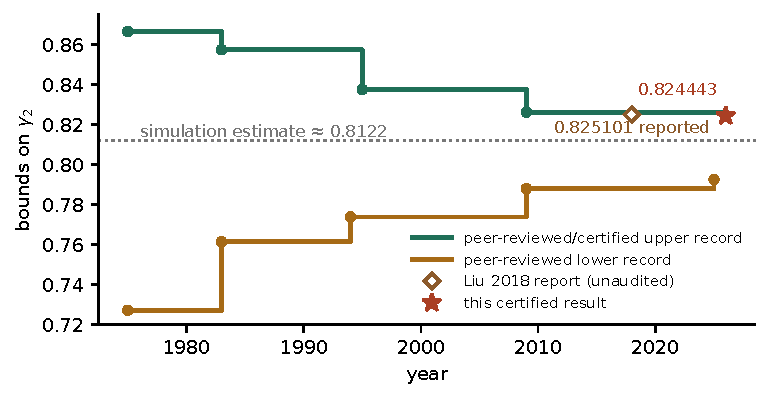
\includegraphics[width=0.70\linewidth]{fig_history.pdf}
  \caption{Peer-reviewed/certified bounds on $\gamma_2$, with Liu's 2018 unaudited report shown separately. This work improves both the previous certified upper record and the reported value.}
  \label{fig:history}
\end{figure}

\section{Result}

\begin{theorem}
$\displaystyle \gamma_2 \;\le\; \frac{824443}{1000000} \;=\; 0.824443 \;<\; 0.826280.$
\end{theorem}

The bound improves the previous peer-reviewed/certified record by $0.001837$ and Liu's reported value by $0.000658$. Relative to the lower bound $0.792665992$, it closes $5.46\%$ of the previous certified gap, or $2.03\%$ if the unaudited report is used as the prior upper endpoint.

\section{Method}

Dan\v{c}\'ik and Paterson introduced the finite-automaton and generating-function method for this upper-bound problem \cite{dancik1995}. Lueker developed the finite-history refinement and positive feasible-function certificate used here \cite{lueker2009}. We keep Lueker's mathematics unchanged and push the finite-history calculation to a machine size that was out of reach in 2009. No new mathematics is introduced; the contribution is a verified computation at a scale two history steps beyond Lueker's published calculation, and the engineering that makes that scale fit on one desktop computer.

\textbf{The certificate idea, in plain words.} The finite-state machine reads grouped minimal-match pairs rather than raw characters from the two strings. A history-$h$ state stores two length-$h$ string suffixes together with two length-$h$ boundary-difference vectors from the LCS dynamic-programming table. Lueker proved that this finite-history machine covers the canonical minimal-match decompositions needed by the Dan\v{c}\'ik--Paterson generating-function argument. His equation~(41) and Theorem~3.3 show that if one can exhibit a vector $v$ of positive numbers, one entry per accepting state, a weight $0<z<\tfrac12$, and a number $0<\lambda<1$ such that a single linear inequality
\[
A_z\, v \;\le\; \lambda\, v
\]
holds coordinate-by-coordinate (where $A_z$ is the machine's transition operator with matches weighted by $z$), then
\[
\gamma_2 \;\le\; \frac{2\log(2z)}{\log \lambda}.
\]
The vector $v$ is the proof-carrying certificate. Its correctness does not depend on how it was found: anyone can recheck the inequality row by row. The cited covering theorem and a faithful construction of its finite machine are separate obligations.

\textbf{Finding the vector.} Larger $h$ gives a stronger bound but exponentially more states. We work at $h=10$: 400{,}253{,}317 states after reduction, with $2(2h-1)=38$ transition columns. The vector is found by power iteration (repeatedly applying $A_z$ and renormalizing), run for 113 sweeps. Two things make this fit in 128\,GB of memory: states are stored once per class of Lueker's simultaneous bit-complement symmetry (the top/bottom exchange is deliberately \emph{not} quotiented, because the canonical tie-breaking in the state encoding does not respect it), and the vector is held in 32-bit fixed-point integers, so the feasibility test is a statement about integers rather than floats. The shipped log records a one-sweep scan of 19 distinct rational $z$ values, using a vector already optimized at $z=3209/10000$; that scan selected $3209/10000$. Because the candidates were not independently converged, we treat the scan only as a local heuristic and make no claim that this $z$ is optimal or that the logged differences measure an unbiased neighbour advantage.

\textbf{Checking the vector.} The claim $\gamma_2 \le 824443/1000000$ reduces, after clearing denominators, to integer comparisons: the feasibility inequality at every one of the 400 million states, and one comparison of logarithms carried out with exact rational enclosures. A deliberate negative control confirms the certificate is sharp: the same vector does \emph{not} prove the next smaller six-decimal target $0.824442$.

\begin{figure}[t]
  \centering
  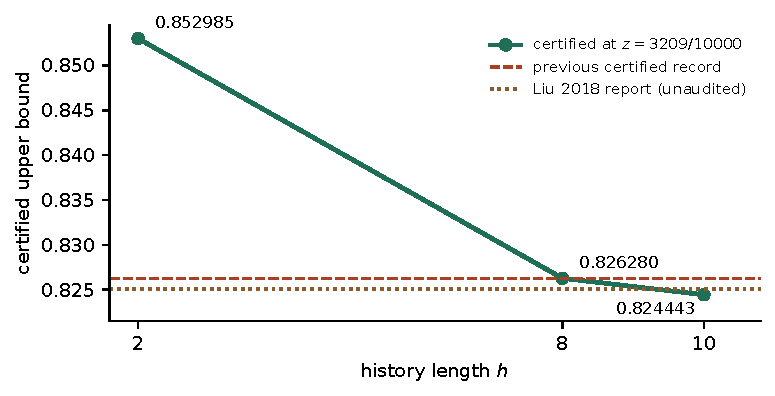
\includegraphics[width=0.70\linewidth]{fig_scaling.pdf}
  \caption{Certified bounds at the fixed value $z=3209/10000$. The $h=8$ point reproduces Lueker's previous certified record (our calibration gate), and $h=10$ gives the new bound. Liu's unaudited report is shown as a separate reference line.}
  \label{fig:scaling}
\end{figure}

\section{Reproducibility}
\label{sec:repro}

Reproducibility is the point of this paper, so we describe the artifact exactly as it ships.

\textbf{What the verifier is.} \texttt{verify\_upper.py} is a single script that re-checks the claim from the stored certificate. It uses NumPy and Numba to apply the operator across 400 million states at reasonable speed; it is not a pure standard-library program. Every inequality that \emph{decides} the claim, however, is evaluated in Python integers and \texttt{Fraction}s: the per-state feasibility test is an integer comparison $S_i \le \Lambda V_i$ against the $\Lambda$ pinned in the script, and the final comparison $2\log(2z)/\log\lambda \le 824443/1000000$ is decided by exact rational enclosures of both logarithms with an explicit remainder bound. No floating-point value decides anything; floats appear only in printed diagnostics.

\textbf{What re-checking costs.} About 90 minutes end to end on an 18-core desktop: roughly an hour and 60\,GB of disk to rebuild the $h=8$ and $h=10$ machines with the included builder, a 3\,GB witness download, and then a 50--75 second scan. The often-quoted ``72 seconds'' is only that final scan.

\textbf{What the verifier checks.} The proof-critical default authenticates the $h=10$ graph and witness checkpoint, enforces witness positivity, declared scale, and successor-index closure, checks the feasibility inequality at every one of the 400{,}253{,}317 states, decides the exact rational log comparison, and asserts that no artifact was modified. An explicit \texttt{--with-provenance} mode additionally authenticates the saved certificate and primary-source PDF when supplied, validates the machine-sizing record, hash-chained sweep log, exact rescale lineage, and $h=8$ calibration, and runs three diagnostics: a negative control (the same witness does \emph{not} prove $0.824442$), a sharpness control (the calibration does not prove better than Lueker's published $0.826280$), and an adversarial control (a deliberately corrupted witness \emph{is} rejected). These optional checks establish lineage and diagnostic confidence; they are not premises of the certificate inequality.

\textbf{What the certificate cannot vouch for.} The theorem quantifies over the $h=10$ machine, so the machine's own correctness is a separate obligation, and hash-pinning authenticates bytes rather than semantics. The dangerous direction is a spurious rejection: the operator drops rejected columns from the row sum, so a legitimate transition wrongly marked as rejecting would understate $A_z$ and make the bound look better than it is. We therefore validate the builder against an independent pure-Python transcription of Lueker's Figure~7 (\texttt{upper\_oracle.py}) in two ways, via \texttt{verify\_graph\_oracle.py}: exhaustively for $h \le 6$ (every state, every column, up to 1.98 million transitions at $h=6$), and by uniformly sampling states of the actual $h=10$ machine and recomputing their complete 38-column rows with the oracle. Both agree with zero mismatches. This is strong evidence rather than proof: the sample covers a small fraction of the machine, and a common-mode misreading of Figure~7 shared by the builder and the oracle would escape both. The $h=8$ calibration reproducing Lueker's published constant is independent evidence against exactly that failure mode.

\textbf{Contents of the release.} The verifier, the certificate ($v$, $z$, $\lambda$, hashes), the graph builder and power iteration used to produce it, the independent oracle and declarative proof contract, exhaustive bounded and mutation tests, the campaign log restricted to the authenticated sweep records, and this manuscript.

\section{Lower-bound scale context}

For scale context, a separate lower-bound run from the campaign returned the exact ratio
\[
\frac{21{,}902{,}062}{27{,}728{,}247}=0.789882678122\ldots,
\]
which rounds to $0.789883$ at six decimal places, at memory length $\ell=17$. The peer-reviewed lower record $0.792665992$ was computed at $\ell=21$ using an external-memory implementation \cite{soiffer2025}. The lower-bound run and its supporting artifacts are not part of this release, so the ratio is provided only as scale context and not as independently replayable evidence here.

\section{Discussion}

The certified interval for $\gamma_2$ is now $[0.792665992,\, 0.824443]$. The builder's sizing heuristic multiplies the largest exact state count by 9 per additional history step, projecting 3{,}602{,}279{,}853 states at $h=11$; no complete $h=11$ closure was built, so this and all dependent memory figures are projections. At that projected size, two 32-bit witness vectors would occupy about $28.8$\,GB. The recorded $103.1$\,GB figure is the projected breadth-first-search hash table, not a transition graph; a dense 42-column uint32 transition array would occupy about $605.2$\,GB before the state array. A future matrix-free implementation could avoid that dense transition storage, but a complete $h=11$ build and certificate remain substantial unperformed work. More broadly, this result shows that a single desktop machine, driven by AI agent loops under a strict discipline --- reproduce the previous certified record first, search with floats, certify with integers, ship a standalone verifier --- can improve a fifty-year-old quantity.

\section{Author contributions}
\label{sec:contributions}

We state authorship plainly rather than leaving it to be inferred. Ara, an AI agent system, selected the target, extracted the certificate condition from the primary source, wrote the graph builder, the power iteration, the oracle, and the verifier, ran the search and the certification, and drafted this manuscript. Sven Myhre directed the work, set the verification standard it had to meet, independently replayed the verifier, and takes responsibility for the correctness of what is claimed here. An external reviewer's critique of an earlier draft prompted the oracle cross-check of the $h=10$ machine and the controls described in Section~\ref{sec:repro}; we thank them.

\begin{thebibliography}{9}
\footnotesize
\setlength{\itemsep}{0.25em}

\bibitem{chvatal1975}
V.~Chv\'atal and D.~Sankoff.
\newblock Longest common subsequences of two random sequences.
\newblock \emph{Journal of Applied Probability}, 12(2):306--315, 1975.

\bibitem{steele1986}
J.~M. Steele.
\newblock An Efron--Stein inequality for nonsymmetric statistics.
\newblock \emph{Annals of Statistics}, 14(2):753--758, 1986.

\bibitem{boutet1999}
J.~Boutet de Monvel.
\newblock Extensive simulations for longest common subsequences.
\newblock \emph{European Physical Journal B}, 7:293--308, 1999.

\bibitem{lueker2009}
G.~S. Lueker.
\newblock Improved bounds on the average length of longest common subsequences.
\newblock \emph{Journal of the ACM}, 56(3):1--38, 2009.

\bibitem{dancik1995}
V.~Dan\v{c}\'ik and M.~Paterson.
\newblock Upper bounds for the expected length of a longest common subsequence of two binary sequences.
\newblock \emph{Random Structures \& Algorithms}, 6(4):449--458, 1995.
\newblock \url{https://doi.org/10.1002/rsa.3240060408}.

\bibitem{liu2018}
Q.~Liu.
\newblock \emph{Topics on the Longest Common Subsequences: Simulations, Computations, and Variance}.
\newblock PhD dissertation, School of Mathematics, Georgia Institute of Technology, 2018.
\newblock \url{https://hdl.handle.net/1853/60772}.

\bibitem{soiffer2025}
D.~Soiffer, A.~Salls, C.~Miller, D.~Reichman, G.~N. S\'ark\"ozy, and G.~T. Heineman.
\newblock Improved lower bounds on the expected length of longest common subsequences.
\newblock In \emph{2025 IEEE International Symposium on Information Theory (ISIT)}, pages 1--6, 2025.
\newblock \url{https://doi.org/10.1109/ISIT63088.2025.11195592}; extended preprint: arXiv:2407.10925.

\end{thebibliography}

\end{document}
